\documentclass[aspectratio=1610,12pt,notheorems]{beamer}

\usepackage[utf8x]{inputenc} \usepackage[russian]{babel}
\usepackage{amsmath,amssymb,amsthm,mathtools}
\usepackage{graphicx,caption,subcaption}
\usepackage{hyperref,natbib}
\usepackage{tikz,xcolor,colortbl,makecell}
\usepackage{algorithm,algpseudocode}
\usepackage{qrcode}

\usetikzlibrary{arrows,backgrounds,patterns,%
	matrix,shapes,fit,calc,shadows,plotmarks,snakes}

\theoremstyle{plain}
\newtheorem{theorem}{Теорема}
\newtheorem{lemma}[theorem]{Лемма}

\theoremstyle{definition}
\newtheorem{definition}{Определение}
\newtheorem{problem}{Задача}

\usetheme[height=0.97cm]{Rochester}
\usecolortheme{dolphin}

\definecolor{hard}{RGB}{145,55,55}
\definecolor{mnsgold}{RGB}{240,235,220}

\setbeamercolor{headline}{bg=hard,fg=mnsgold}
\setbeamercolor*{frametitle}{parent=headline}

\setbeamercolor{structure}{fg=hard}
\setbeamercolor{subsection in head/foot}{bg=white,fg=hard}
\setbeamercolor{section in head/foot}{bg=hard,fg=mnsgold}
\setbeamercolor{block title}{bg=hard,fg=mnsgold}

\setbeamertemplate{navigation symbols}{}

\parskip=2.6mm
\def\ll{\left(} \def\rr{\right)}
\def\lag{\left\langle} \def\rag{\right\rangle}

\definecolor{failpos}{RGB}{230,30,20}
\definecolor{initpos}{RGB}{30,20,220}
\definecolor{turna}{RGB}{100,240,110}
\definecolor{turnb}{RGB}{250,140,110}

\newcommand{\vseper}{\vphantom{$\int_{0_0}^{0^0}$}}

\newcommand{\singlepayoff}[2]{\tikz{
	\draw (0,0) node{\vseper #1}; \draw (0.8,0.8) node{\vseper #2};
}}

\newcommand{\rowdescription}[1]{\tikz{
	\draw (0,0) node{\vseper #1}; \draw (0,0.8) node{\vseper};
}}

\newcommand{\coldescription}[1]{\tikz{
	\draw (0,0) node{\vseper}; \draw (0.8,0) node{\vseper #1};
}}

\newcommand{\myref}[2]{\href{#1}{\texttt{\underline{#2}}}}

\def\mitem{\medskip\item}
\def\ps{\\ [0.65cm]} \linespread{1.16}
\def\fram#1#2{\begin{frame}\frametitle{#1}#2\end{frame}}
\def\usl#1#2{\begin{block}{#1} #2 \end{block} \medskip\pause}
\def\uslnp#1#2{\begin{block}{#1} #2 \end{block} \medskip}
\def\mov#1#2{\begin{scope}[xshift = #1 cm] #2 \end{scope};}

\def\divsby{\mathrel{\rlap{.}\rlap{\raisebox{0.55ex}{.}}\raisebox{1.1ex}{.}}}
\definecolor{starvert}{RGB}{110,175,230}
\newcommand{\vfi}{\varphi}
\newcommand{\litem}{\vspace{0.5cm}\item}

\newcommand{\nkstar}[2]{
	\foreach \i in {1,...,#1} {\draw[thick] (90 + 360 * \i / #1 : 3.5)
		-- (90 + 360 * \i / #1 + 360 * #2 / #1 : 3.5);}
	\foreach \i in {1,...,#1} {\fill[starvert] (90 + 360 * \i / #1 : 3.5) circle[radius=0.16cm];}
}

\title{\bfseries Davenport—Schinzel Sequences}

\author{Boris Zolotov, Algo Lunch}

\institute[\ ]{\ }

\date{December 9, 2020}

%%%%%%%%%%%%%%
%%%%%%%%%%%%%%

\begin{document}

\frame{\titlepage}

\begin{frame} \frametitle{Definition}

\begin{block}{\vspace*{-3ex}}
	D—S sequence of order $n$: no {\it sebsequences} $a \ldots$ $b\ldots$ $a \ldots$ $b\ldots$ of length $n+2$
\end{block}

	Motivation: lower envelope of continuous functions that coincide at no more than $n$ points.

\begin{center}
	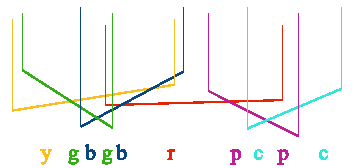
\includegraphics[width=0.5\textwidth]{algolunch/ds-segments}
\end{center}

	For each segment we can construct the set of functions. \vspace{1cm}

\end{frame}

\begin{frame} \frametitle{Voronoi diagrams and the beach line}
\begin{center}
	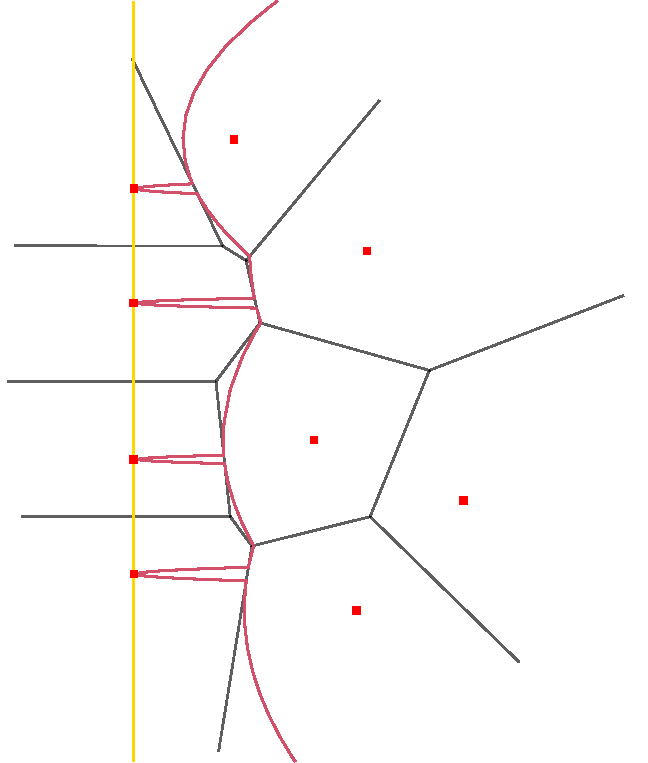
\includegraphics[width=0.48\textwidth]{algolunch/example}
\end{center}
\end{frame}

\begin{frame} \frametitle{Changes and cost model}

\begin{block}{\vspace*{-3ex}} \vspace{-2.2ex}
	$$\text{\bf Insert} (a_{k+1})$$
\end{block}

\begin{block}{\vspace*{-3ex}} \vspace{-2.2ex}
	$$\text{\bf Relabel} (a_j, a_{k+1}, S)$$
\end{block}

	$$\text{\bf Delete} \colon\quad a_{k+1}a_{k+1}\ 
	    \rightarrow\ a_{k+1}$$

\end{frame}

\begin{frame} \frametitle{Two Inserts per step}

\begin{block}{\vspace*{-3ex}}
Restate that maximal length of D—S sequence is $2n-1$ in «amortized fashion».
\end{block}

\begin{itemize}
	\item Between two occurences of letter $x$ some letters are «trapped». \medskip
	\item We give 2 pennies to each letter initially. \medskip
	\item Idea: each letter pays for its father. \medskip
	\item Invariants: each letter with $k$ instances receives at least $k-1$ pennies from its descendants, can pay one to its father. \medskip
	\item Finally, all the occurences are paid for.
\end{itemize} \vspace{1cm}
\end{frame}

\begin{frame} \frametitle{Location of Relabels}
\begin{block}{\vspace*{-3ex}}
	Letters that we relabel form a union of subtrees with their roots located on the same level and having a common father.
\end{block}

\begin{figure} \centering
	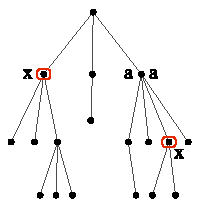
\includegraphics[width=0.34\textwidth]{algolunch/sametree} \hspace{1.5cm}
	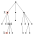
\includegraphics[width=0.34\textwidth]{algolunch/samelevel}
\end{figure}
\end{frame}

\begin{frame} \frametitle{What happens to the tree when we relabel} \vspace{1cm}

	We can think that relabels happen from top down: this order does not disrupt the D—S property.

\begin{figure} \centering
	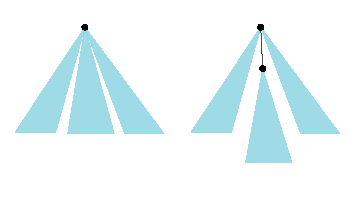
\includegraphics[width=0.7\textwidth]{algolunch/firstpush}
\end{figure}
\end{frame}

\begin{frame} \frametitle{What happens to the tree when we relabel} \vspace{1cm}

	When we relabel vertices on lower levels we make their children our clidren. We can think of it as a subtree contracted into a single vertex.

\begin{figure} \centering
	
\includegraphics[width=0.7\textwidth]{algolunch/furtpush}
\end{figure}
\end{frame}

\begin{frame} \frametitle{Size and potential}
	Define size of the node as number of its children $+1$.

\begin{block}{\vspace*{-3ex}} \vspace{-1.8ex}
	$$2n\ \ge\ \sum\limits_v \mathrm{size}\, (v)\ \ge\ \mathrm{length}\, (S)$$ \vspace{-1ex}
\end{block}

Define the potential function as
\begin{block}{\vspace*{-3ex}} \vspace{-1.8ex}
	$$\sum\limits_v \min \left( \mathrm{size}\, (v), \sqrt{n} \right)$$ \vspace{-1ex}
\end{block}

\end{frame}

\begin{frame} \frametitle{$\sqrt{n}$ Relabels amortized}
Each time we relabel we steal someone's children or delete a node. Let $s$ be the number of children transferred.

\begin{align*}
	& s + \Phi_{\text{new}} - \Phi_{\text{old}} \le \\
\le\ 	& s + \sqrt{n} - (s - \sqrt{n}).
\end{align*}

\end{frame}

\begin{frame} \frametitle{But is that really $\sqrt{n}$?}
\begin{figure}
	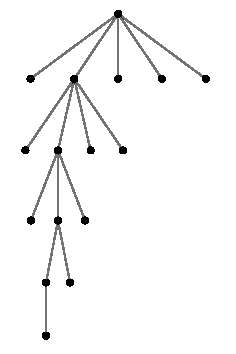
\includegraphics[height=0.92\textheight]{algolunch/sqrtn}
\end{figure}
\end{frame}

\end{document}
